\section{Technical evaluation}
\label{sec:technical_evaluation}

The technical evaluation of this chapter includes several experiments that are 
carried out aiming to test the performance of the adaptation process. One of 
the most important developed modules of AdaptUI is the Pellet reasoning 
engine port for Android. This module requires extra effort in the evaluation, as 
leads the whole adaptation process. Besides, several other experiments are 
presented. Thus, in the following sections these experiments and their results 
are detailed:

% This section gathers several experiments regarding the technical part of the 
% evaluation. Within this section the following experiments are included:

\begin{enumerate}[label=\alph*)]
  \item First, Section~\ref{sec:performance_evaluation} presents a series 
  of experiments regarding the performance of \textit{Pellet4Android} in 
  comparison with Pellet for Java. For more details of the 
  \textit{Pellet4Android} mobile reasoning engine see 
  Section~\ref{sec:pellet4android}.
  
  \item Second, AdaptUI is compared to another user adaptation solution: 
  Imhotep. This is detailed in Section~\ref{sec:imhotep_comparison}.
  
  \item Next, several scenarios are presented to evaluate the adaptation 
  process of AdaptUI. Besides, the Imhotep's user adaptation framework is also
  compared. The scenarios and their details are given in 
  Section~\ref{sec:scenarios}.
  
  \item Finally, $5$ developers with experience in developing Android based 
  applications have evaluated the provided \acs{api}. This experiment is detailed
  in Section~\ref{sec:developers}.
\end{enumerate}


\subsection{Performance evaluation for Pellet and Pellet4Android}
\label{sec:performance_evaluation}

During this section different experiments are presented in order to 
discuss the results of using mobile reasoning engines. In our case we evaluate 
the reasoning performance of \textit{Pellet4Android}, the Android based version 
of Pellet ported for AdaptUI. To do so, this evaluation considers Pellet, the 
desktop Java based reasoning engine, to make a comparison between the 
performance results of both solutions. This evaluation has been divided into 
three different experiments:

\begin{enumerate}
  \item The first experiment consists in using the default AdaptUIOnt ontology 
  version with both reasoning engines. When loading the ontology several rules 
  are processed and triggered. As a result of this experiment the  
  corresponding performance results are compared.
  
  \item For the second experiment the ABox axioms set of the AdaptUIOnt 
  ontology is increased. The ABox gathers the knowledge about the 
  individuals, including concepts and roles assertions, and individuals 
  equality and inequality~\citep{krotzsch_description_2012}. In other words, 
  it describes the attributes of instances (or individuals), the roles between 
  instances, and other assertions about instances regarding their class 
  membership with the TBox concepts~\citep{abox_tbox}. The ABox, RBox and TBox 
  belong to the \ac{owl} 2 Description Logic (DL). As for these experiments several 
  modifications have been carried out in these axiom sets, a more concrete 
  description of the concepts represented by each set is detailed in 
  Table~\ref{tbl:dl_terminology}. Hence, increasing the number of individuals   
  might result into difference performance results comparing both platforms.
  
  \item Next, the \ac{swrl} axioms set of the AdaptUIOnt ontology is modified by 
  increasing its axioms. This axiom set collects axioms related to the rules 
  included in the ontology. Therefore, this experiment focuses on the reasoning 
  capabilities of each version of Pellet.
\end{enumerate}

\begin{table}
 \caption{TBox and ABox components purposes~\citep{abox_tbox}.}
 \label{tbl:dl_terminology}
 \footnotesize
 \centering
\begin{tabular}{l l l}
  \hline 
  \textbf{ABox} 				&  \textbf{TBox} \\
  \hline 
  Membership assertions, either as concepts or  & Definitions of the concepts and properties of the 	\\
  as roles. 					& controlled vocabulary.				\\
  Attributes assertions. 			& Declarations of concept axioms or roles.		\\
  Linkages assertions that capture the above	& Inferencing of relationships, be they transitive, 	\\
  but also assert the external sources for 	& symmetric, functional or inverse to another 		\\
  these assignments. 				& property.						\\
  Consistency checking of instances.		& Equivalence testing as to whether two classes or 	\\
  Satisfiability checks, which imply that the	& properties are equivalent to one another.		\\
  conditions of instance memberships are met.	& Subsumption, which is checking whether one 		\\
						& concept is more general than another.			\\
						& Satisfiability, which is the problem of checking 	\\
						& whether a concept has been defined (is not an 	\\
						& empty concept).					\\
						& Classification, which places a new concept in  	\\
						& the proper place in a taxonomic hierarchy of 		\\
						& concepts.						\\
						& Logical implication, which is whether a generic 	\\
						& relationship is a logical consequence of the		\\ 
						& declarations in the TBox.				\\
						& Infer property assertions implicit through the 	\\
						& transitive property.					\\	
\hline
\end{tabular}
\end{table}

% For these experiments several tables and the corresponding charts are included,
% showing the results obtained during the tests. In these tables the ontology 
% triples, ABox and \ac{swrl} axioms sets, mean, median and deviation are shown. The
% triples are obtained by a SPARQL query (see Listing~\ref{lst:fuseki}). On the
% other hand the axioms are requested through the \ac{owl}-API.
% 
% \lstset{label=lst:fuseki, language=java, basicstyle=\footnotesize, frame=single,
% keywordstyle=\color{blue}, captionpos=b, caption={SPARQL query for obtaining the
% number of triples of the ontology. Between the $WHERE$ braces there is:
% $?s$, which represents the subject; $?p$, representing the predicate; and $?o$,
% which represents the object.}, breakatwhitespace=false, breaklines=true}
% \begin{lstlisting}
%   SELECT (COUNT(*) AS ?no) WHERE { ?s ?p ?o  }
% \end{lstlisting}


The cited experiments have been performed using two different types of devices 
have been used. The ones running Pellet have been launched using a desktop 
environment. On the contrary, as \textit{Pellet4Android} is an Android based 
version of the reasoning engine, several mobile devices have been tested. The 
characteristics of all the devices used for these experiments are detailed in 
Table~\ref{tbl:devices_specs}. 

\begin{table}
 \caption{Execution platforms software and hardware main specifications. The \ac{ram}
 memory is measured in \ac{gb} and the \ac{cpu} processor in \ac{ghz}.}
 \label{tbl:devices_specs}
 \footnotesize
 \centering
\begin{tabular}{l l l l}
  \hline 
 \textbf{Device} 		& \multicolumn{2}{c}{\textbf{Hardware}} 	
& \textbf{Software}	\\
				& \textbf{\ac{ram}} & \textbf{\ac{cpu}} 			
& \textbf{\ac{os}} 		\\
    \hline 
  Acer TravelMate 8481  	& 8.0	& Quad-core 1.60 Intel® 	 	
& Ubuntu 13.10 		\\
				& 	& Core™ i5-2467M			
& (64 bits)		\\
  Samsung Galaxy SIII Mini	& 1.0 	& Dual-core 1.0, Cortex-A9	 	
& Android 4.1.2 	\\
  Samsung Galaxy SIII 		& 1.0 	& Quad-core 1.4, Cortex-A9 		
& Android 4.3   	\\
  Samsung Nexus 10 		& 2.0 	& Dual-core 1.7, Cortex-A15 		
& Android 4.4.2 	\\
\hline
\end{tabular}
\end{table}

The mobile devices shown in the previous table have not been chosen arbitrarily.
As can be seen in Figure~\ref{fig:android_market}, at February 2014 the global
spread of Samsung devices represent the 65\% share of all Android devices.

\begin{figure}
\centering
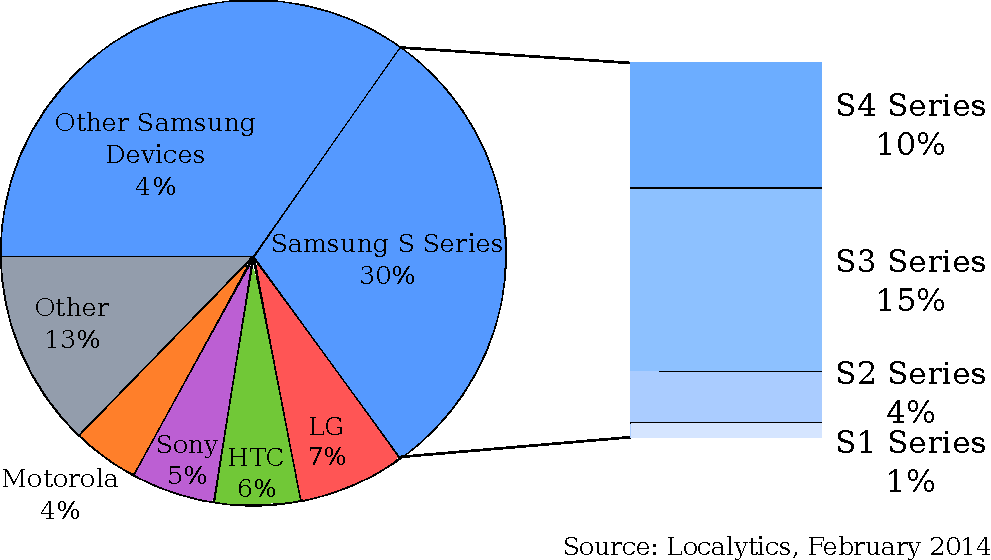
\includegraphics[width=0.75\textwidth]{android_market.pdf}
\caption{Global Android share~\citep{samsung_share_2014}. As this pie chart
illustrates, Samsung devices represent the 65\% of the Android worldwide market
share.}
\label{fig:android_market}
\end{figure}

According to the explanation of this section, in the following lines each 
experiment is described and evaluated. First, the default AdaptUIOnt reasoning 
performance comparing Pellet and \textit{Pellet4Android} is introduced in 
Section~\ref{sec:eval_default_ont}. Next, these reasoning engines are 
tested using a modification of the default ontology, increasing the ABox axioms 
set. This experiment is described in Section~\ref{sec:eval_abox}. 
Finally, the AdaptUIOnt default ontology's \ac{swrl} axioms set is increased to 
evaluate the performance of both reasoning engines when dealing with larger 
sets of rules (see Section~\ref{sec:eval_swrl}).


\subsubsection{Using the default AdaptUIOnt ontology}
\label{sec:eval_default_ont}

In this experiment the default version of the AdaptUIOnt ontology is used as 
input of the reasoning engines in order to evaluate their performance. As 
AdaptUIOnt has been designed to be a light ontology to be available to be used 
with mobile reasoning engines, this experiment shows how \textit{Pellet4Android} 
performs in comparison with the the results obtained by Pellet in a desktop 
environment. These results are shown in Table~\ref{tbl:eval_default_ont}.

\begin{table}
 \caption{Pellet and \textit{Pellet4Android} comparison loading the default 
AdaptUIOnt ontology.}
 \label{tbl:eval_default_ont}
 \footnotesize
 \centering
  \begin{tabular}{l l r r r r r r}
  \hline 
  &  & \multicolumn{2}{c}{\textbf{Axioms}} & 
  \multicolumn{3}{c}{\textbf{Results}}	\\
  \textbf{Device} & \textbf{Triples}& \textbf{ABox} & \textbf{\ac{swrl}}
  & \textbf{Mean} & \textbf{Median} & \textbf{Deviation}	\\
  \hline 
  Acer laptop	& 2,779	& 37  & 13 & 0.946 & 0.951 & 0.017	\\
  (Pellet)							\\
  Galaxy SIII Mini& 2,779& 37 & 13 & 2.764 & 2.737 & 0.127	\\
  (\textit{Pellet4Android})					\\
  Galaxy SIII	& 2,779	& 37  & 13 & 1.649 & 1.652 & 0.076	\\
  (\textit{Pellet4Android})					\\
  Nexus 10	& 2,779	& 37  & 13 & 5.147 & 5.122 & 0.205	\\
  (\textit{Pellet4Android})					\\
  \hline
\end{tabular}
\end{table}

Figure~\ref{fig:pellet_default} illustrates the differences of using Pellet or
\textit{Pellet4Android} when loading the default ABox and \ac{swrl} axiom sets in 
AdaptUIOnt. As is shown in Figure~\ref{fig:pellet_default} and in 
Table~\ref{tbl:eval_default_ont}, the performance of Pellet for Java 
environments is better in any case if we compare it with the Android based 
version. However, and although there are several differences depending on the 
used mobile device, the differences are small. This is specially remarkable in 
the case of the Samsung Galaxy SIII. This device performs a remarkable 1.649 
seconds, which is just approximately 0.7 slower than Pellet for Java.

\begin{figure}
\centering
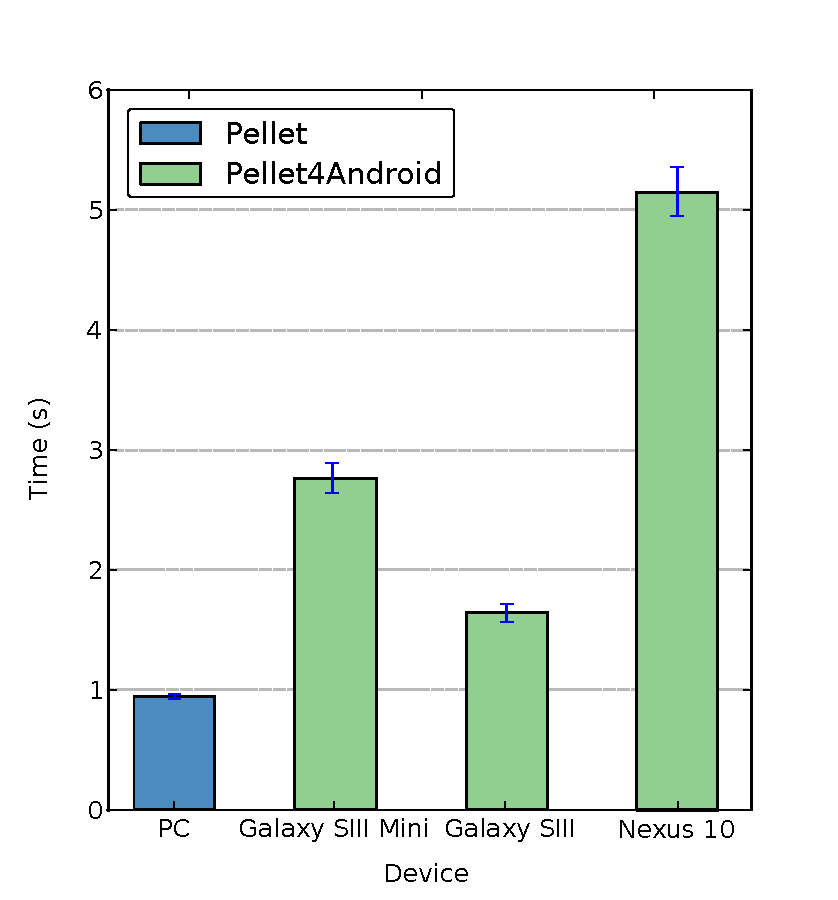
\includegraphics[width=0.75\textwidth]{pellet_default.pdf}
\caption{Pellet and \textit{Pellet4Android} performance comparison using the
default AdaptUIOnt ontology.}
\label{fig:pellet_default}
\end{figure}

\subsubsection{Incrementing the ABox axioms set}
\label{sec:eval_abox}

In this case the experiment consists in incrementing the ABox axioms set of 
the AdaptUIOnt ontology. As stated before, the ABox describes the attributes of 
instances, the roles between instances, and other assertions about instances 
regarding their class membership with the TBox concepts~\citep{abox_tbox}. 
The modification of the ABox has been carried out by incrementing the amount of 
instances in 5,000, 10,000, 15,000 and finally reaching 20,000 instances. Thus, 
with this experiment we want to evaluate how increasing the number of 
individuals might result into a performance penalization, specially in the case 
of \textit{Pellet4Android}. Table~\ref{tbl:eval_abox} shows the results of this
experiment.

\begin{table}
 \caption{Pellet and \textit{Pellet4Android} comparison loading the AdaptUIOnt 
ontology with an increment in the ABox axiom set.}
 \label{tbl:eval_abox}
 \footnotesize
 \centering
  \begin{tabular}{l l r r r r r r}
  \hline 
  &  & \multicolumn{2}{c}{\textbf{Axioms}} & 
  \multicolumn{3}{c}{\textbf{Results}}	\\
  \textbf{Device} & \textbf{Triples}& \textbf{ABox} & \textbf{\ac{swrl}}
  & \textbf{Mean} & \textbf{Median} & \textbf{Deviation}	\\
  \hline 
  Acer laptop & 12,779 & 5,000  & 13 & 3.014 & 3.012 & 0.034	\\  
  (Pellet)    & 22,779 & 10,000 & 13 & 3.903 & 3.905 & 0.052	\\
	      & 32,779 & 15,000	& 13 & 4.228 & 4.231 & 0.036	\\
	      & 42,779 & 20,000 & 13 & 4.539 & 4.541 & 0.042	\\
  \hline	      
  Galaxy SIII Mini& 12,779& 5,000& 13& 59.412& 59.508& 0.708	\\
  (\textit{Pellet4Android}) & 22,779 & 10,000 & 13 & 30.321 & 30.327 & 0.347 \\
	      & 32,779 & 15,000	& 13 & 87.957 & 87.018 & 1.108 	\\
	      & 42,779 & 20,000	& 13 & 183.882&183.879 & 2.101	\\
  \hline	      
  Galaxy SIII & 12,779 & 5,000	& 13 & 36.336 & 36.194 & 0.668	\\
(\textit{Pellet4Android})& 22,779 & 10,000 & 13	& 16.471 & 16.439 & 0.288\\
		& 32,779 & 15,000 & 13 & 45.387	& 45.593 & 0.729\\
		& 42,779 & 20,000 & 13 & 97.151	& 97.440 & 1.120\\
  \hline		
  Nexus 10	& 12,779 & 5,000  & 13 & 14.171 & 14.428 & 0.525\\
(\textit{Pellet4Android})& 22,779 & 10,000 & 13 & 9.024 & 9.065 & 0.291\\
		& 32,779 & 15,000 & 13 & 17.944& 17.969  & 0.496\\
		& 42,779 & 20,000 & 13 & 32.070	& 32.019 & 0.588\\
  \hline
\end{tabular}
\end{table}

Figure~\ref{fig:pellet_abox} illustrates the differences between Pellet and
\textit{Pellet4Android} when loading the AdaptUIOnt ontology with an increment 
applied to the ABox axioms set. As is shown in the chart (accordingly with
Table~\ref{tbl:eval_abox}) the performance of Pellet for Java environments 
keeps being better in comparison with the Android based version. While Pellet
maintains its performance under 5 seconds, Android devices require much more
time to perform the same reasoning. In fact, specially the Samsung Galaxy SIII 
Mini mobile device requires more than 180 seconds to evaluate the corresponding
20,000 instances, while the Samsung Galaxy SIII needs approximately 97 seconds 
and the Nexus 10 not more than 32.

\begin{figure}
\centering
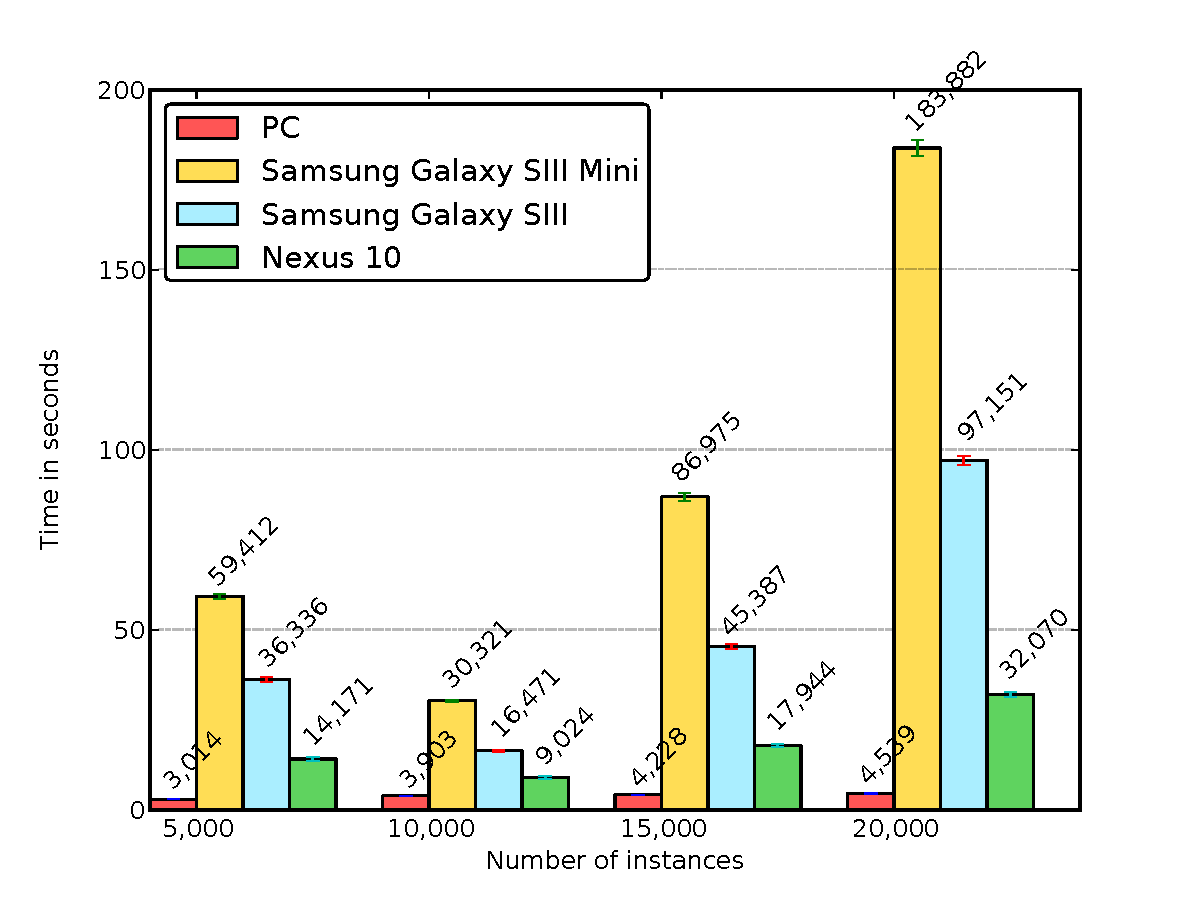
\includegraphics[width=0.95\textwidth]{pellet_abox.pdf}
\caption{Pellet and \textit{Pellet4Android} performance comparison using the
AdaptUIOnt ontology increasing the ABox axioms set.}
\label{fig:pellet_abox}
\end{figure}

\subsubsection{Incrementing the \ac{swrl} axioms set}
\label{sec:eval_swrl}

Finally, this last experiment consists in incrementing the \ac{swrl} axioms set of 
the AdaptUIOnt ontology, which collects the axioms related to the rules
included in the ontology. Using an amount of 5,000, 10,000, 15,000 and 
finally 20,000 rules we aim to evaluate how increasing the number of rules 
penalize the performance of Pellet, specially in the case of 
\textit{Pellet4Android}. Table~\ref{tbl:eval_swrl} shows the results of this
experiment.

\begin{table}
 \caption{Pellet and \textit{Pellet4Android} comparison loading the AdaptUIOnt 
ontology with an increment in the \ac{swrl} axiom set.}
 \label{tbl:eval_swrl}
 \footnotesize
 \centering
  \begin{tabular}{l l r r r r r r}
  \hline 
  &  & \multicolumn{2}{c}{\textbf{Axioms}} & 
  \multicolumn{3}{c}{\textbf{Results}}	\\
  \textbf{Device} & \textbf{Triples}& \textbf{ABox} & \textbf{\ac{swrl}}
  & \textbf{Mean} & \textbf{Median} & \textbf{Deviation}	\\
  \hline 
  Acer laptop & 82,779  & 37 & 5,013  & 4.770 & 4.732 & 0.141	\\
  (Pellet)    & 162,779 & 37 & 10,013 & 6.327 & 6.296 & 0.164 	\\
	      & 242,779	& 37 & 15,013 & 7.427 & 7.194 & 0.444 	\\
	      & 322,779	& 37 & 20,013 & 8.147 & 8.117 & 0.105	\\
  \hline
 Galaxy SIII Mini& 82,779 & 37 & 5,013  & 96.878  & 96.988  & 0.109 \\
(\textit{Pellet4Android}) & 162,779& 37 & 10,013 & 101.656 & 101.899 & 0.322 \\
	      & 242,779	& 37 & 15,013 & 243.981	& 244.011 & 0.298 \\
	      & 322,779	& 37 & 20,013 & 331.433	& 331.894 & 0.110 \\	
	\hline      
  Galaxy SIII & 82,779	& 37 & 5,013 & 84.121 & 84.121 & 0.869	\\
(\textit{Pellet4Android})& 162,779 & 37	& 10,013 & 74.248 & 74.103 & 0.250\\
		& 242,779 & 37 & 15,013	& 209.431 & 208.628 & 1.699 \\
		& 322,779 & 37 & 20,013	& 216.005 & 216.077 & 1.202 \\
\hline
  Nexus 10	& 82,779 & 37 & 5,013 & 22.317 & 22.471	& 0.333 \\
		& 162,779& 37 & 10,013& 45.193 & 44.736	& 1.312	\\
		& 242,779& 37 & 15,013& 85.543 & 88.134 & 5.490	\\
		& 322,779& 37 & 20,013& 107.151& 106.131& 2.749	\\
  \hline
\end{tabular}
\end{table}

Figure~\ref{fig:pellet_swrl} illustrates the differences between Pellet and
\textit{Pellet4Android} when running the different sets of \ac{swrl} axioms of the 
AdaptUIOnt ontology. As is shown in the chart it takes more time to evaluate the 
set of rules than the instances. In fact, the scale of the Y axis reaches 350 
seconds, while in Figure~\ref{fig:pellet_abox} the maximum mean reaches less 
than 200 seconds.

\begin{figure}
\centering
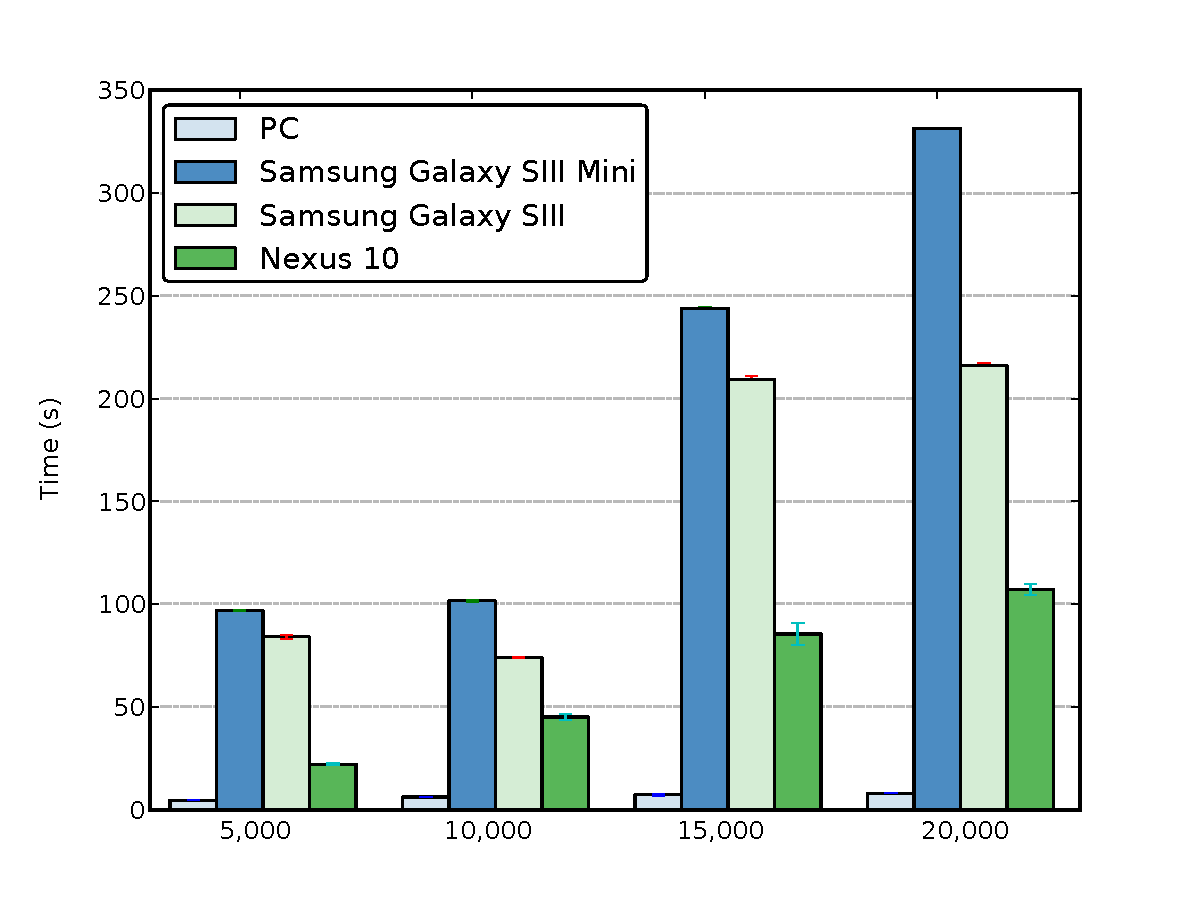
\includegraphics[width=0.95\textwidth]{pellet_swrl.pdf}
\caption{Pellet and \textit{Pellet4Android} performance comparison using the
AdaptUIOnt ontology increasing the \ac{swrl} axioms set.}
\label{fig:pellet_swrl}
\end{figure}

\subsubsection{Discussion}
\label{sec:performance_discussion}

During these experiments, and as is shown in Table~\ref{tbl:eval_default_ont}, 
Table~\ref{tbl:eval_abox} and Table~\ref{tbl:eval_swrl}, neither the TBox or 
RBox axioms sets have been modified. These collections belong to what is called 
the terminology knowledge in \ac{owl} 2, and it does not affect the performance of 
the reasoning process. Hence, the TBox and the RBox contain 266 and 22 axioms 
respectively during the experiments.

On the contrary, sets of 5,000, 10,000, 15,000 and 20,000 axioms have been added
to the ABox and \ac{swrl} axioms sets to demonstrate the performance penalization of 
when using large axioms sets with the tested reasoning engine. These 
modifications of the AdaptUIOnt ontology have been performed through several 
Python scripts, which have modified the corresponding default 
\textit{adaptui.owl} file.


\subsubsection{Conclusions}
\label{sec:performance_conclusions}

These results demonstrate that, although managing semantics in mobile devices is
possible, they still lack of more appropriate capabilities to perform reasoning
tasks. Nevertheless, \textit{Pellet4Android} is a good approximation of a 
reasoner to run on mobile devices. A native Pellet for Android port written in 
C++ would probably improve these results. But one of the AdaptUIOnt ontology's 
benefits is its lightness. Using less than 400 axioms, this ontology is able to 
model a full adaptation domain, remarking the user and his/her capabilities, the 
surrounding environment and the device characteristics. The results shown in 
Table~\ref{tbl:eval_default_ont} show how \textit{Pellet4Android} responses 
properly when dealing with the AdaptUIOnt ontology. However, more efforts in 
mobile reasoners would benefit these systems.

% Repasar bien
Regarding the ABox collection of axioms, the first conclusion that is extracted
from the results shown in Table~\ref{tbl:eval_abox} is that Pellet running in a 
PC has a very optimal response. For example, increasing the number of instances 
to almost 20,000 instances just reduces the response time in around 4 seconds 
(see Figure~\ref{fig:pellet_abox}). Increasing the ABox slows down the final 
performance, incrementing the number of seconds for loading the ontology. On 
the contrary, running this experiment in the mobile devices reveals a lack of 
efficiency. First, each device's hardware capabilities are taken into account. 
The first mobile device, the Samsung Galaxy SIII~Mini needs around 2.764 
seconds for loading the default AdaptUI ontology with its 37 ABox and 13 \ac{swrl} 
axioms. This same case takes 1.649 seconds in the Samsung Galaxy SIII and 5.147 
seconds in the Nexus 10. Although these figures might be appear to be enough 
considering we are dealing with limited Hardware, by increasing them in the 
same way that it has been done with the Acer laptop results into unmanageable
time responses. For instance, loading 5,032 ABox axioms takes 3.014 seconds for
the laptop and Pellet, for the Samsung Galaxy SIII Mini it takes 59.412 seconds,
36.336 seconds for the Samsung Galaxy SIII and 14.171 seconds for the Nexus 10. 

Nevertheless, these differences are more significant when dealing with the \ac{swrl}
axioms set. In this case, although Pellet's performance does not exceed 9 
seconds, the differences with the ABox axioms set are much bigger regarding
\textit{Pellet4Android}. In the best case, the Nexus 10 needs around 22 seconds
to reason over a 5,000 rules, while the Samsung Galaxy SIII Mini needs more 
than 90. This depicts the existing differences of performance depending on the
Android device we choose.